We will now calculate the mismatch for a fully-coherent search given the
random walk in phase, frequency, and spin-down rate defined in the previous
section.

Let us begin by expanding the metric-mismatch summation from Eqn.~\eqref{eqn:
mismatch}.  Writing the summations explicitly, we have
\begin{align}
\mutilde & = g_{\alpha\beta i j}\dl^{\alpha i}\dl^{\beta j}  \\
&=\s{i=1}{\Nsd}\s{j=1}{\Nsd}g_{\alpha\beta i j}\dl^{\alpha i}\dl^{\beta j}  \\
&= \s{i=1}{\Nsd}g_{\alpha\beta i i}\dl^{\alpha i}\dl^{\beta i}
+ \s{i=1}{\Nsd} \s{\substack{j=1\\ j \ne i}}{\Nsd} g_{\alpha \beta ij}\dl^{\alpha i}\dl^{\beta j}.
\end{align}
The summation has been intentionally split into terms for which the two
subdomains are the same and those for which they are different. The metric when
the reference time is at the beginning of each subdomain is given by
Eqn.~\eqref{eqn: metric equal subdomains tref 0}. By considering the metric for
the two cases, we can write the two distinct components as
\begin{equation}
g_{\alpha\beta ij} = \left\{
\begin{array}{cc}
g_{\alpha\beta}^{\mathrm{E}} & \textrm{ if } i =j \\
g_{\alpha\beta}^{\mathrm{NE}} & \textrm{ if } i  \ne j
\end{array}\right.  .
\end{equation}
Then the fully-coherent metric-mismatch can be calculated from
\begin{align}
\mutilde &= \s{i=1}{\Nsd}g_{\alpha\beta}^{\mathrm{E}}\dl^{\alpha i}\dl^{\beta i}
+ 2\s{i=1}{\Nsd} \s{j=1}{i-1} g_{\alpha \beta}^{\mathrm{NE}}\dl^{\alpha i}\dl^{\beta j} .
\label{eqn: mismatch sep}
\end{align}

\subsection{Writing the parameter offsets in terms of normal distributions}
Equations~\eqref{eqn: f offset} and \eqref{eqn: phi
offset} give the offsets as functions of the offsets in higher order
parameters. In order to calculate statistical values, we now write these in terms of
the normal distributions from which the random walks are constructed.
Substituting Eqn.~\eqref{eqn: delta fdot n} into Eqn.~\eqref{eqn: f offset} and using the summation properties defined
in Appendix~\ref{sec: summation identities}, we have
\begin{align}
\Delta \f_{i}  & = \s{j=1}{i}\tn \f_{j}
+ \s{j=1}{i-1}\s{k=1}{j}\tn \fdot_{k} \dT ,  \\
& = \s{j=1}{i}\tn \f_{j}
+ \s{j=1}{i-1}(i-j)\tn \fdot_{j} \dT .
\label{eqn: delta f n}
\end{align}
Similarly, substituting this equation into Eqn.~\eqref{eqn: phi offset} we
have
\begin{align}
\begin{split}
\Delta\phi_{i} & = \s{j=1}{i}\tn \phi_{j}
+ 2\pi \left(\s{j=1}{i-1}\Delta\f_{j}\dT
+ \frac{1}{2}\s{j=1}{i-1}\Delta\fdot_{j}\dT^{2}\right) \\
& = \s{j=1}{i}\tn \phi_{j} + 2\pi\left(\s{j=1}{i-1}\left(\s{k=1}{j}\tn\f_{k}
+ \s{k=1}{j-1}(j-k)\tn\fdot_{k}\dT\right)\dT
 + \frac{1}{2}\s{j=1}{i-1}\s{k=1}{j}\Delta\fdot_{k}\dT^{2} \right)  \\
& = \s{j=1}{i}\tn \phi_{j} + 2\pi\left(\s{j=1}{i-1}(i-j)\tn\f_{j}\dT
 + \s{j=1}{i-1}\s{k=1}{j-1}(j-k)\tn\fdot_{k}\dT^{2}
 + \frac{1}{2}\s{j=1}{i-1}(i-j)\Delta\fdot_{j}\dT^{2} \right)  \\
& = \s{j=1}{i}\tn \phi_{j} + 2\pi\left(\s{j=1}{i-1}(i-j)\tn\f_{j}\dT
 + \frac{1}{2}\s{j=1}{i-1}\left(\left(i-j\right)\left(i-j-1)\right)
 + (i-j)\right)\tn\fdot_{j}\dT^{2}\right)  \\
& = \s{j=1}{i}\tn \phi_{j} + 2\pi\left(\s{j=1}{i-1}(i-j)\tn\f_{j}\dT
 + \frac{1}{2}\s{j=1}{i-1}(i-j)^{2}\tn\fdot_{j}\dT^{2}\right)
\end{split}
\label{eqn: delta phi n}
\end{align}

\subsection{Taking the expectation}

In Eqn.~\eqref{eqn: delta fdot n}, Eqn.~\eqref{eqn: delta f n},
Eqn.~\eqref{eqn: delta phi n} we have written the parameter space offsets
(which are to be used in calculating the mismatch) purely in terms of the
random walk distributions $\tn \phi_i$, $\tn \f_i$, and $\tn \fdot_i$. We can
calculate the mismatch exactly given a set of random walk jumps by inserting
these into Eqn.~\eqref{eqn: mismatch sep}. However, since we are dealing with
statistical quantities, we can instead infer the behaviour of the mismatch
under the random walk by taking an expectation.

Inserting Eqn.~\eqref{eqn: delta fdot n}, Eqn.~\eqref{eqn: delta f n},
Eqn.~\eqref{eqn: delta phi n}  in Eqn.~\eqref{eqn: mismatch sep} yields a
number of terms with all the permutations of two terms from $[\tn \phi, \tn \f,
\tn \fdot]$. Taking the expectation, all the cross-correlated terms, such as
$\tn\phi_{i}\tn \fdot$, will have an expectation of zero since the steps of the
random walk are independent. The only non-vanishing terms are given by
\begin{align}
E[\tn\phi_{i}\tn\phi_{j}] &= \delta_{ij}\sigP, &
E[\tn\f_{i}\tn\f_{j}] &= \delta_{ij}\sigF,&
E[\tn\fdot_{i}\tn\fdot_{j}] &= \delta_{ij}\sigS,
\end{align}
After some simplification we find that the mismatch is given by
\begin{align}
\begin{split}
E[\mutilde]   = &  \frac{A_{\phi}}{6} \left(\Nsd - \frac{1}{\Nsd}\right)
+ \frac{\pi^{2} A_{{f}}}{30}\left(4 \Nsd^{3} + 5 \Nsd^{2} + \frac{1}{\Nsd}\right)\\
 & +  \frac{\pi^{2} A_{{\dot{f}}}}{3780} \left(66 \Nsd^{5} - 21 \Nsd^{3} + 105 \Nsd^{2}
 + 217 \Nsd + 63 - \frac{94}{\Nsd}\right),
\end{split}
\label{eqn: expectation}
\end{align}
where
\begin{equation}
	A_{\phi} = \sigP \;\;\;\;\;
    A_{\f} = \sigF\Delta T^{2} \;\;\;\;\;
    A_{\fdot} = \sigS\Delta T^{4},
\end{equation}
define three `activity parameters'.

Recalling that $\Nsd=\Tobs/\Delta T$, Eqn.~\eqref{eqn: expectation} makes
predictions for the leading order
scaling of the three random walks with the observation period
\begin{equation}
E[\mutilde]_{\mathrm{PN}} \sim \sigP \frac{\Tobs}{\Delta T}, \hspace{10mm}
E[\mutilde]_{\mathrm{FN}} \sim \sigF \frac{\Tobs^{3}}{\Delta T}, \hspace{10mm}
E[\mutilde]_{\mathrm{SN}} \sim \sigS \frac{\Tobs^{5}}{\Delta T}.
\label{eqn: scalings}
\end{equation}

These results are a function both of the observation span $\Tobs$ and the
random walk model parameters $\sigP, \sigF, \sigS$ and $\Delta T$. In
Appendix~\ref{sec: physical interpretation of the monthly ephemeris}, we showed
that for a compound Poisson process random walk, the variance after a duration
$\Delta T$ scaled as $\sigma^{2} \propto \Delta T$. This means that the leading
order scalings in Eqn.~\eqref{eqn: scalings} are insensitive to how the random
walk is parameterised: changing $\Delta T$ produces a corresponding change in
$\sigma^{2}$ such that the leading order mismatch remains the same for a fixed
observation time.

\subsection{Verifying the results}

We can observe the leading order scaling of Eqn.~\eqref{eqn: scalings}
directly and verify the predictions made by Eqn.~\eqref{eqn: expectation} by
comparing with exact numerical results. That is, using the signal injection and
recovery tools developed in Section~\ref{sec: narrow-band method} of
Chapter.~\ref{sec: timing noise in cgw} we simulate signals undergoing a random
walk and calculate the corresponding mismatch (no minimisation step is done
here, this is discussed in the next section). In particular, we perform three
Monte Carlo studies for a random walk in the phase, frequency, and spin-down
rate and in each case compare the simulated results with the analytic
prediction. The results are shown in Figure~\ref{fig: rw I} and demonstrate good
agreement between the simulation means and the prediction of Eqn.~\eqref{eqn:
expectation}.

\begin{figure}[ht]
\centering
\subfloat[Random walk in phase]{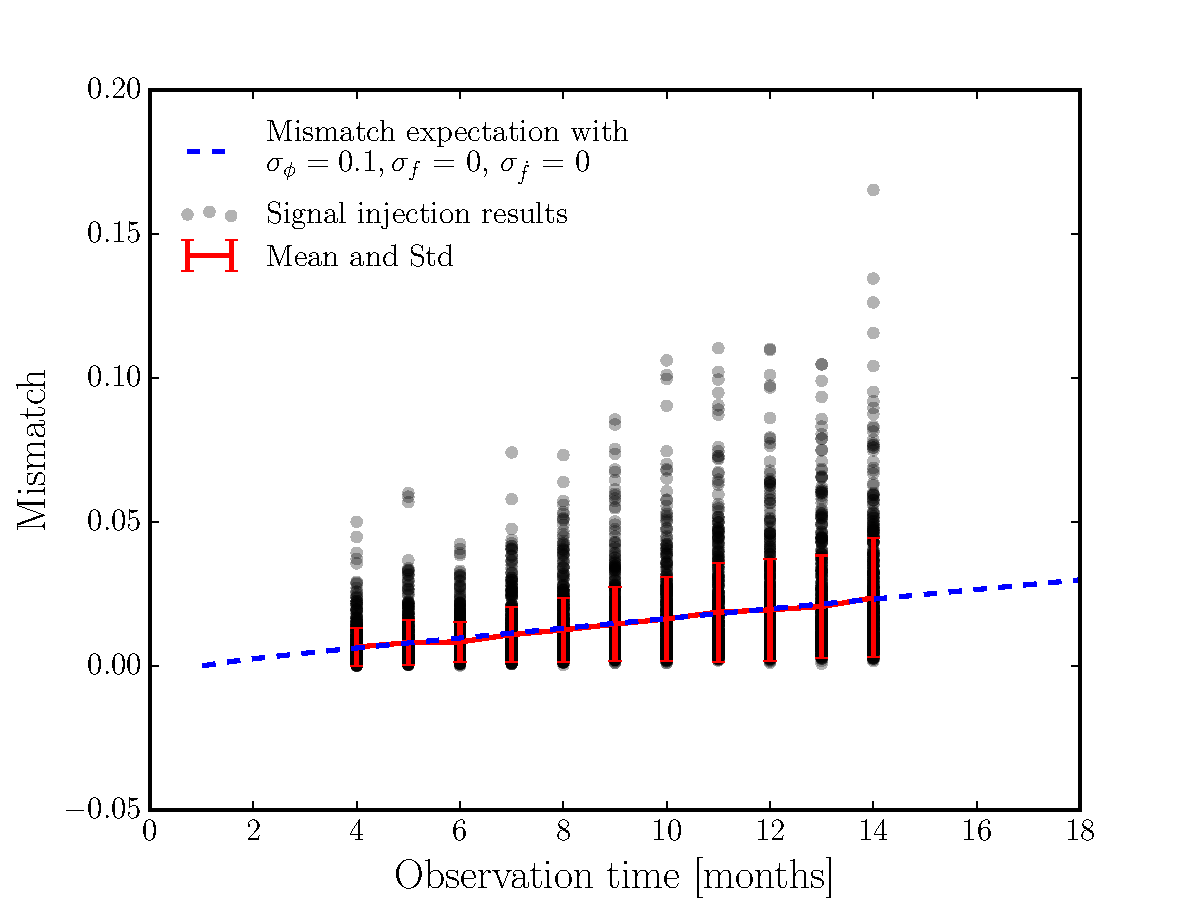
\includegraphics[width=0.5\textwidth]{ExpectationPhase}}
\subfloat[Random walk in frequency]{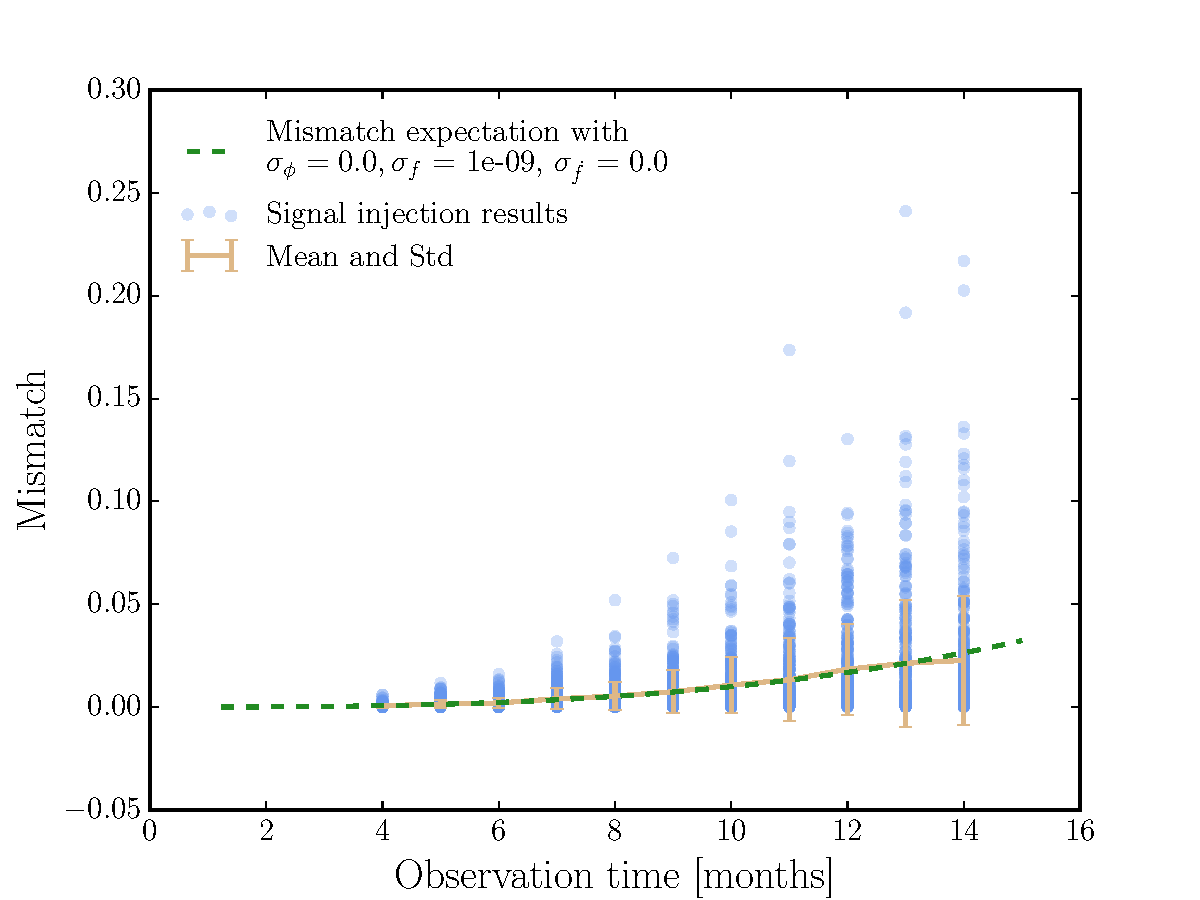
\includegraphics[width=0.5\textwidth]{ExpectationFrequency}}\\ \subfloat[Random walk in spin-down]{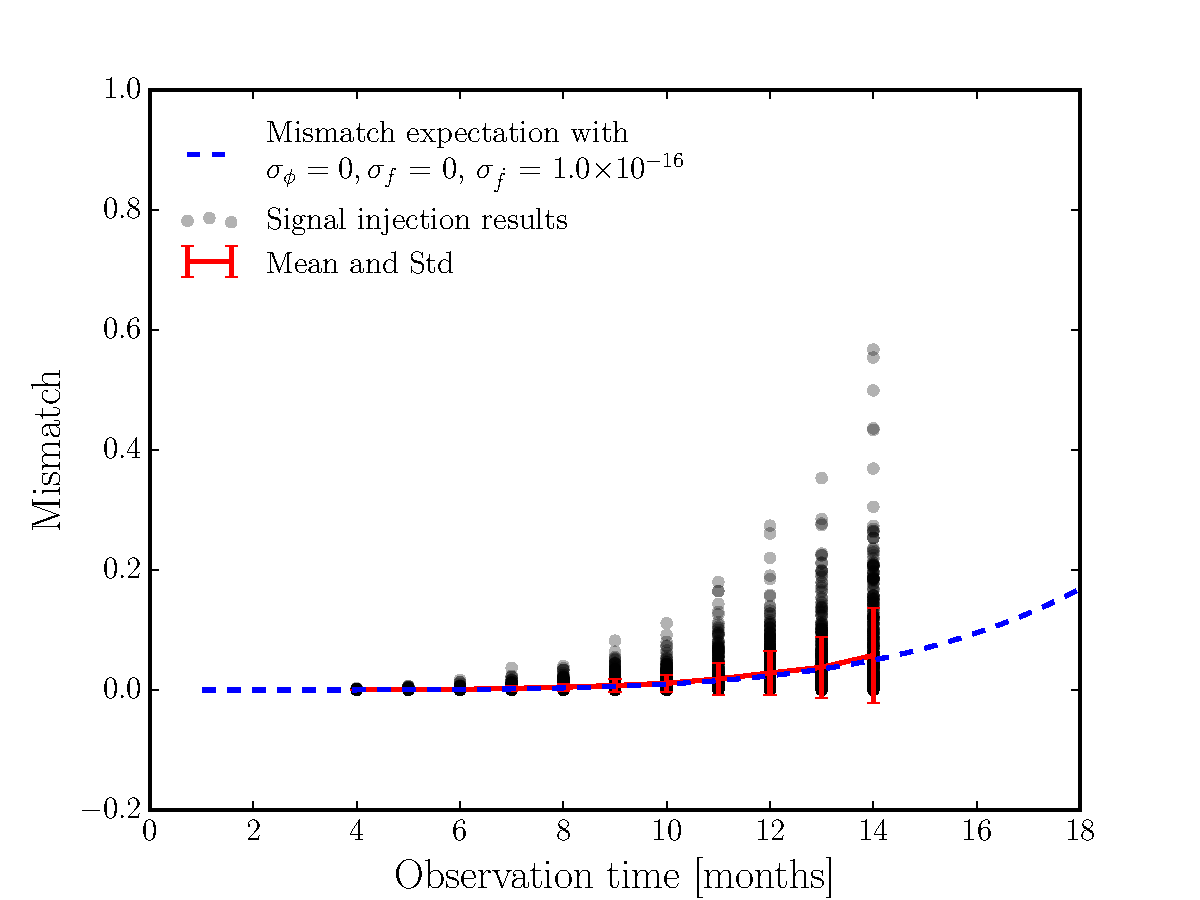
\includegraphics[width=0.5\textwidth]{ExpectationSpindown}}
\caption{A comparison of Monte Carlo numerical simulated mismatch with the prediction
of Eqn.~\eqref{eqn: expectation} for a random walk in the phase, frequency,
and spin-down rate.}
\label{fig: rw I}
\end{figure}

\subsection{Implied scalings}

